\documentclass[12pt]{article}

\input{../../_assets/preambulo.tex}


\begin{document}

    % 1. Foto de fondo
    % 2. Título
    % 3. Encabezado Izquierdo
    % 4. Color de fondo
    % 5. Coord x del titulo
    % 6. Coord y del titulo
    % 7. Fecha

    
    \input{../../_assets/portada}
    \portadaExamen{ffccA4.jpg}{Geometría III\\Examen XVII}{Geometría III. Examen XVII}{MidnightBlue}{-8}{28}{2025}{Roxana Acedo Parra}

    \begin{description}
        \item[Asignatura] Geometría III.
        \item[Curso Académico] 2025-26.
        \item[Grado] Doble Grado en Ingeniería Informática y Matemáticas.
        \item[Grupo] Único.
        \item[Profesor] Antonio Ros Mulero.
        \item[Descripción] Convocatoria extraordinaria.
        \item[Fecha] 16 de febrero de 2026.
        \item[Duración] 3 horas.
    \end{description}
    \newpage
    
    \begin{ejercicio}[2,5 puntos]En el plano euclídeo $\bb{R}^2$ consideramos el segmento $AB$, con $A=(a,0)$ y $B=(0,b)$, $a, b>0$.
        \begin{figure}[H] 
        \centering
            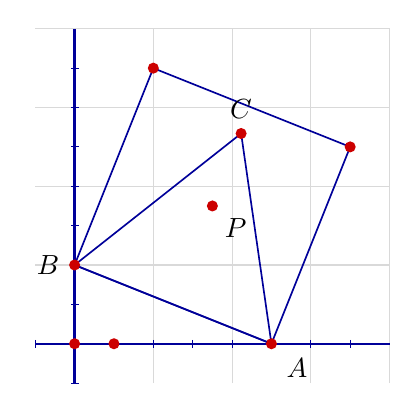
\begin{tikzpicture}[x=0.5cm, y=0.5cm]
                \draw[lightgray!60, thin] (-1,-1) grid (8,8);
    
                \draw[blue!60!black, thick] (-1,0) -- (8,0);
                \draw[blue!60!black, thick] (0,-1) -- (0,8);
            
                \foreach \x in {-1, 1, 2, 3, 4, 5, 6, 7}
                    \draw[blue!60!black] (\x, 0.1) -- (\x, -0.1);
                \foreach \y in {-1, 1, 2, 3, 4, 5, 6, 7}
                    \draw[blue!60!black] (0.1, \y) -- (-0.1, \y);
            
                \path (5,0) coordinate (A);
                \path (0,2) coordinate (B);
            
                \path (4.23, 5.34) coordinate (C);
            
                \path (2,7) coordinate (E);
                \path (7,5) coordinate (D);
            
                \path (3.5, 3.5) coordinate (P);
    
                \draw[blue!60!black, semithick] (A) -- (B) -- (E) -- (D) -- cycle;
            
                \draw[blue!60!black, semithick] (A) -- (B) -- (C) -- cycle;
            
                \fill[red!80!black] (A) circle (2pt);
                \fill[red!80!black] (B) circle (2pt);
                \fill[red!80!black] (C) circle (2pt);
                \fill[red!80!black] (D) circle (2pt);
                \fill[red!80!black] (E) circle (2pt);
                \fill[red!80!black] (P) circle (2pt);
            
                \fill[red!80!black] (0,0) circle (2pt);
                \fill[red!80!black] (1,0) circle (2pt);
    
                \node[below right=2pt] at (A) {$A$};
                \node[left=2pt] at (B) {$B$};
                \node[above=2pt] at (C) {$C$};
                \node[below right=1pt] at (P) {$P$};
            \end{tikzpicture}
        \end{figure}

        \begin{enumerate}[label=(\alph*)]
            \item Calcular las coordenadas del centro $P$ del cuadrado de lado $AB$ contenido en el primer cuadrante.
            \item Calcular las coordenadas del tercer vértice $C$ del triángulo equilátero de lado $AB$.
        \end{enumerate}
    \end{ejercicio}


    \begin{ejercicio}[2,5 puntos]En el espacio euclídeo $\bb{R}^3$ consideramos las rectas
    $$r_1\equiv\begin{cases}x=0\\ y=1\end{cases} \quad r_2\equiv\begin{cases}y=0\\ z=2\end{cases}$$
        \begin{enumerate}[label=(\alph*)]
            \item Razonar que $r_1$ y $r_2$ se cruzan y calcular las ecuaciones de la recta perpendicular común.
            \item Encontrar la expresión matricial de un movimiento rígido que lleve $r_1$ en $r_2$ y $r_2$ en $r_1$.
            \item Demostrar que la aplicación siguiente es un movimiento rígido. Clasificarlo y encontrar sus elementos geométricos.
            \Func{f}{\bb{R}^3}{\bb{R}^3}{(x,y,z)}{(-y,z+2,-x+1)}
        \end{enumerate}
    \end{ejercicio}
    

    \begin{ejercicio}[2,5 puntos]~ 
        \begin{enumerate}[label=(\alph*)]
            \item En el plano euclídeo $\bb{R}^2$, encontrar la ecuación de la cónica $\cc{C}$ que pasa por los cinco puntos $A(0,0)$, $B(1,0)$, $C(0,1)$, $D(1,1)$, $E(2,3)$.
            \item Calcular la ecuación de la recta tangente a $\cc{C}$ en el punto $D$.
            \item Dada la cónica $4x^2-y^2-8x-2y+2=0$ clasificarla y encontrar sus elementos geométricos.
        \end{enumerate}
    \end{ejercicio}

    \begin{ejercicio}[2,5 puntos]En el espacio afín $\bb{R}^3$, consideramos la cuádrica
    $$\cc{Q}\equiv2x^2+y^2+az^2+2xy-2y-2az+a=0, \quad a\in\bb{R}.$$
        \begin{enumerate}[label=(\alph*)]
            \item Calcular su centro.
            \item Clasificarla para cada valor de $a$.
        \end{enumerate}
    \end{ejercicio}

\end{document}